% !TEX encoding = UTF-8
% !TEX TS-program = pdflatex
% !TEX root = computabilità e algoritmi.tex
% !TEX spellcheck = it-IT

\subsection{Calcolo della durata e del lavoro}\label{calcolo-della-durata-e-del-lavoro}

Il calcolo del lavoro è semplice, basta andare a contare tutte le
porzioni di codice sequenziale.

Per calcolare la durata è necessario tenere conto se due attività
possono essere eseguite in parallelo

\begin{figure}[htbp]
\centering
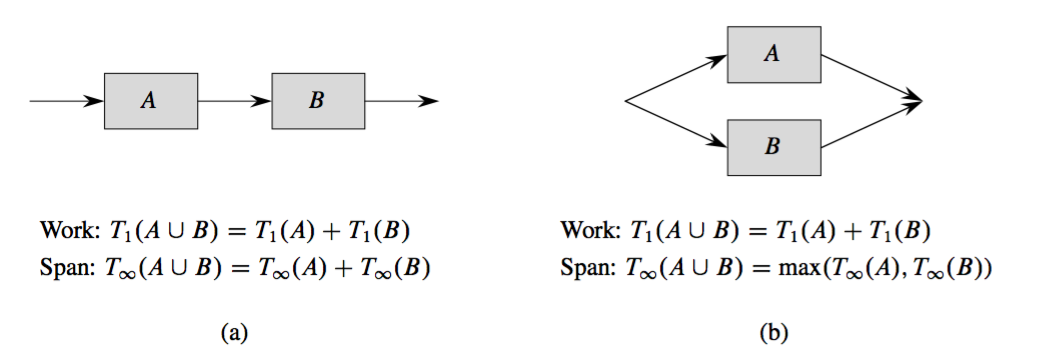
\includegraphics{./notes/immagini/l25-fig1.png}
\caption{}
\end{figure}

Se due computazioni devono essere eseguite in sequenza la durata è la
somma dei Tinf delle due compitazioni. Se invece possono essere eseguiti
in parallelo, la durata è il massimo dei due Tinf.

\subsection{Loop paralleli}\label{loop-paralleli}

Moltiplicazione di un vettore per una matrice di dimensione \emph{nxn}

\begin{verbatim}
\Function{MatVec}{$A,x$}
    \State $n \gets A.rows$
    \State $y\gets Vec(n)$
    \State \textbf{parallel}
    \For{$i = 1 \text{ to } n$}
        \State $y_i \gets 0$
    \EndFor
    \State \textbf{parallel}
    \For{$i = 1 \text{ to } n$}
         \For{$j = 1 \text{ to } n$}
            \State $y_i \gets y_i + a_{i,j}x_j$
        \EndFor
    \EndFor
\end{verbatim}

Per quanto riguarda il lavoro si ha T1(n) = Tetha(n\^{}2).

La durata invece Tinf(n) si ha che il primo blocco \textbf{parallel} ha
durata Theta(log(n)), perché il ciclo di azzeramento viene ottimizzato
in modo analogo dalla piattaforma parallela in qualcosa di simile:

\begin{verbatim}
Azzera(y,i,j)
if i = j
    y_i = 0
else 
    m = floor(i+j/2)
    spawn azzera(y,i,m)
    azzera(y,m+1,j)
    sync
\end{verbatim}

Il lavoro di questa procedura in funzione di n = j-i+1 è T1(n)= 2T1(n/2)
+ C = Theta(n). Tinf(n) è invece unguale a Tinf(n/2)+C = Theta(log(n))
che deve essere sommata alla durata del blocco, che in questo caso è
costante.

In modo simile a prima il secondo blocco ha complessità Theta(log(n)) +
Theta(n) = Theta(n).

Si ha quindi che quando c'è un parallel c'è sempre una costante log(n)
da sommare alla complessità a causa dell'implementazione del for.

Tinf di tutto l'algoritmo è quindi Theta(n).

\subsection{Race condition}\label{race-condition}

Se l'esecuzione dell'algortimo fornisce sempre lo stesso risultato viene
detto \textbf{deterministico} e questo avviene quando l'ordine di
esecuzione degli strand non è influente sul risultato.

Se invece l'ordine è influente sul risultato si ha che l'agoritmo è
\textbf{non deterministo} e questo può essere causato da delle
\textbf{race condition} ovvero quando due strand eseguiti in paralleli
accedono alla stessa locazione di memoria.

\subsection{Una lezione di scacchi}\label{una-lezione-di-scacchi}

Un algoritmo parallelo è stato progettato per lavorare con p = 32 e con
un T32 = 65 secondi.

Si è poi riusciti a ridurre il tempo di esecuzione a T'32 = 40 secondi.

Tuttavia una volta eseguito il codice con p = 512 la seconda versione
dell'algoritmo è risultata meno performante.

La versione originale aveva T1 = 2048 e Tinf = 1, mentre quella
modificata aveva T'1 = 1024 e Tinf 8. Ovvero la seconda versione ha
dimezzato il lavoro, ma ha aumentato la durata.

Per il programma originale, utilizzando Tp = T1/p + Tinf:

T32 = 2048/32 +1 = 65 T'32 = 1024/32 +8 = 40

mentre

T512 = 2048/512 + 1 = 5 T512 = 1024/512 + 8 = 10

Morale della favola, diminuire il lavoro non sempre porta ad una
riduzione della durata.

\section{Merge Sort}\label{merge-sort}

La versione sequenziale dell'algoritmo prende un array \emph{A} e due
indici \emph{p} e \emph{r} e deve ordinare la porzione dell'array
compresa tra \emph{p} e \emph{r}.

\begin{verbatim}
\Function{MergeSort'}{$A,p,r$}
\If{$p < r$}
    \State $q \gets floor(p+r/2)$
    \State \textbf{spawn } \texttt{MergeSort'}$(A,p,q)$
    \State \texttt{MergeSort'}$(A,q+1,r)$
    \State \textbf{sync}
    \State \texttt{Merge}$(A,p,q,r)$
\EndIf
\EndFunction
\end{verbatim}

Il lavoro T1(n) è Theta(n log(n)) che deriva dalla versione sequenziale
del \texttt{MergeSort}.

La durata è invece uguale ad un tempo costante, più la massima durata
delle chiamata ricorsive (che possono essere considerate uguali) più la
durata del merge, che se viene fatto in modo sequenziale è Theta(n). Si
ha quindi che Tinf = Tinf(n/2) + Theta(n) = Theta(n) (\emph{per il
metodo dell'esperto o qualcosa del genere}).

Il parallelismo di questo algoritmo risulta quindi essere Theta(log(n))
che non risulta essere buono.

\begin{verbatim}
To sort 10 million elements, for example, it might achieve linear speedup on a few processors, but it would not scale up effectively to hundreds of processors.
\end{verbatim}

Per aumentare il parallelismo è necessario rendere parallela anche la
funzione \texttt{Merge}.

\begin{figure}[htbp]
\centering
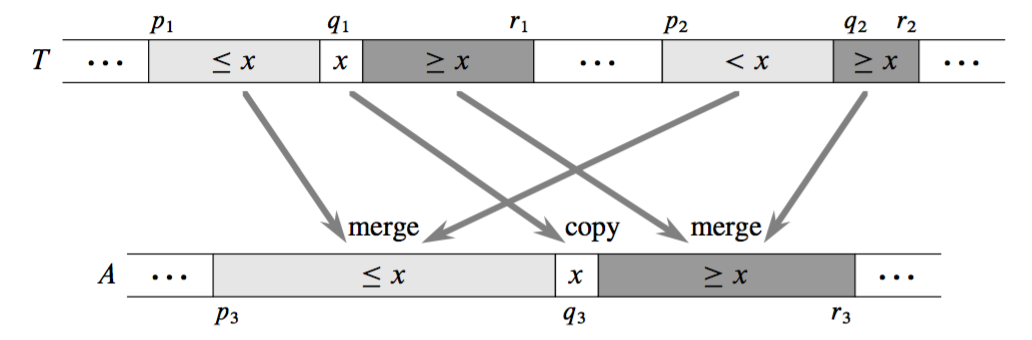
\includegraphics{./notes/immagini/l25-fig2.png}
\caption{}
\end{figure}

Supponiamo che nell'array \emph{T} risultante dalle due chiamate
ricorsive ci siano due porzioni ordinate che vanno rispettaivamente da
\emph{p1} a \emph{r1} e da \emph{p2} a \emph{r2}.

L'idea è quella di prendere la parte più lunga dei due segmenti. Se
questa è lunga 0, sono entrambi vuoti e non è necessario fare niente.

Se invece è più lunga di 0, viene calcolato l'indice \emph{q1} medio,
ovvero l'elemento centrale della sequenza, il quale avrà un certo valore
\emph{x}.

La seconda sequenza può quindi essere divisa in altre due sottosequenze
contenenti solo valori minori di \emph{x} e un'altra con tutti i valori
\emph{\textgreater{}= x}. Il primo elemento \emph{\textgreater{}= x}
avrà un certo indice \emph{q2}. Questo può essere fatto con il binary
search in un tempo logaritmico.

Da notare che \emph{q2} può essere uguale a \emph{p2} se sono tutti
maggiori uguali o a \emph{r2+1} se sono tutti minori.

Si sa quindi che una volta ordinato il vettore, l'elemento \emph{x} si
troverà nella posizione \emph{q3 = p3 + (q1-p1) + (q2-p2)} e può essere
già scritto.

Si possono poi unire ricorsivamente tutti gli elementi minori di
\emph{x}, ovvero quelli che vanno da \emph{p1} a \emph{q1-1} e da
\emph{p2} a \emph{q2-1} , e tutti quelli maggiori uguali di \emph{x},
ovvero quelli che vanno da \emph{q1} a \emph{r1} e da \emph{q2} a
\emph{r2}.

Dal momento che i primmi andranno a finire nelle posizioni da \emph{q3}
a \emph{q3-1} e i secondi andranno a finire nelle posizioni da
\emph{q3+1} a \emph{r3}, le due chiamate ricorsive possono essere
parallelizzate.
